\chapter{実験}
ここでは本研究において行った実験について述べる.

\section{ドライブレコーダー映像を利用した実験}
\subsection{実験内容}
本研究における最初の本実験として,予備実験をもとに実装したシステムを実際にドライブレコーダー映像を使って検証した.
また,strct2depth画面における車のbbox内のG値が100を超えた際に渋滞と判断し,画面左上に「Traffic Jam」という文字列が表示されるようにした.
加えて,映像中に渋滞が判断された回数をフレームごとにJam Counterとして回数を映像中段左に表示されるようにした.

\subsection{使用したデータセット}
本実験にて使用したデータセットは動画投稿サイトYouTubeにて公開されていた高速道路を走行中の映像に加え,私の家族が使用している自家用車に取り付けられたドライブレコーダー映像を用いる.
どの映像も30秒から1分のものであり,常に先行車がある映像を使用した.以下に使用した映像について表で示す.

% ----------------------------------------------------
\begin{table}[htbp]
  \centering
  \begin{scriptsize}
  \begin{tabular}{ccccc}
  \toprule
映像番号 & 時間帯 & 撮影場所 & 車線数 & 動画時間\\
  \midrule
映像1 & 昼間 & 一般道 & 1 & 1分\\
映像2 & 昼間 & 一般道 & 2 & 1分\\
映像3 & 不明 & 高速道路(トンネル) & 2 & 1分 \\
映像4 & 夜間 & 高速道路 & 3 & 30秒\\
  \bottomrule
  \end{tabular}
  \end{scriptsize}
  \caption{使用したデータセット}
  \label{tab:dataset}
\end{table}
% ------------------------------------------------------
\newpage
% 実験1で発生した問題を述べる
\section{実験結果と課題}
ここでは実験1における実験結果について問題と考察を述べる.
まず,実験1における実験結果の一部を以下に示す.
実験結果1〜3の通り,予備実験にて改良したシステムをそのまま用いると,様々な状況で渋滞を誤検出するという問題が発生してしまう.

% --------------------------------------------------
\begin{figure}[htbp]
  \begin{tabular}{c}
    \begin{minipage}{0.33\hsize}
      \begin{center}
   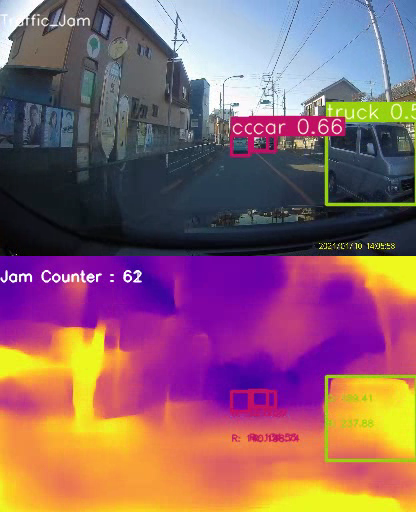
\includegraphics[width=4.5cm]{figs/ex01_01.png}
    \end{center}
  \caption{結果1}
  \label{fig:ex01_01}
\end{minipage}

  \begin{minipage}{0.33\hsize}
  \begin{center}
    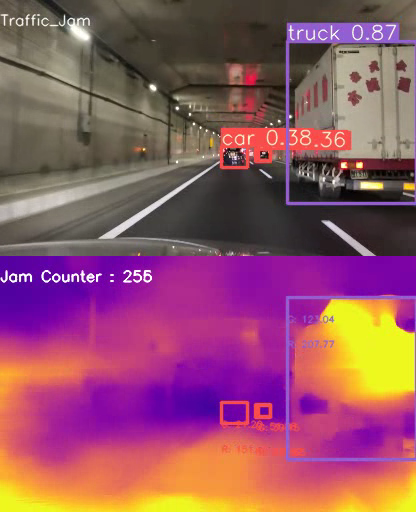
\includegraphics[width=4.5cm]{figs/ex01_02.png}
  \end{center}
  \caption{結果2}
  \label{fig:ex01_02}
\end{minipage}

  \begin{minipage}{0.33\hsize}
  \begin{center}
    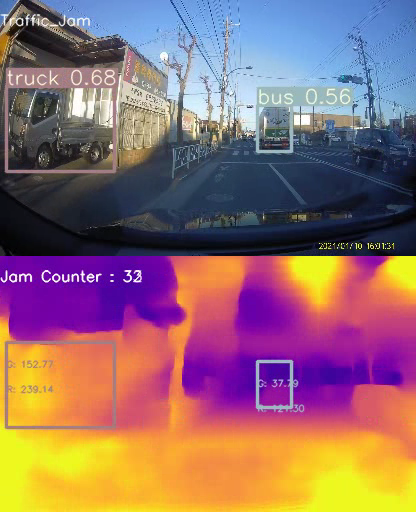
\includegraphics[width=4.5cm]{figs/ex01_03.png}
  \end{center}
  \caption{結果3}
  \label{fig:ex01_03}
\end{minipage}
\end{tabular}
\end{figure}
% ---------------------------------------------------

\figref{fig:ex01_01},\figref{fig:ex01_02},および\figref{fig:ex01_03}の結果からわかるように様々な要因で渋滞の誤検出が起きた.
まず,\figref{fig:ex01_01}においては対向車がドライブレコーダー付きの自動車を横切ってしまうとその際に渋滞と判断してしまう例である.
対向車の存在は渋滞と関係ないのに対し,渋滞と判断してしまうのは正しい判断ではない.
次に,\figref{fig:ex01_02}においては,複数車線がある場合に隣の車線の自動車が近くで走行している際に渋滞だと判断してしいる例である.
先述の対向車のケースとは異なり,隣の車線の混雑は走行車線の混雑と関係がある.
しかし,\figref{fig:ex01_02}のように,先行車との距離があるにもかかわらずたまたま隣で走っていたトラックが近いがために渋滞だと判断してしまうのは正しい判断ではない.
そして,\figref{fig:ex01_03}においては,道路脇に駐車しているトラックを画像検知システムが検知してしまい,渋滞だと判断している例である.
高速道路では稀であるが一般道を走行している際に道路脇に自動車が駐車されているのは珍しいことではなく,またその駐車は渋滞には一切関係がない.
それにもかかわらず渋滞だと判断しているのは正しい判断ではない.
これらの判断ミスのケースは\tabref{tab:dataset}の表にある映像のいずれにおいても頻繁に発生する問題であった.

\subsection{解決アプローチ}
実験1における問題の解決のために対向車,隣車線の自動車および駐車している自動車を検出しないという解決策を取った.
対向車や隣車線の自動車といったものはドライブレコーダー映像において左右の1/3に写っている.
ここに着目し,左右1/3に写っている自動車類の検出をしないように改良した.

\section{改良したシステムを用いた実験}
実験1における解決アプローチを元にプログラムを改良した.
プログラムにおいて処理中の画像の横のサイズは416ピクセルなので,その1/3である138ピクセルの範囲で左右における自動車類を検出しないようにした.

\section{実験結果}
映像中における実験1と同じフレームの画像での実験結果を以下に示す.

% --------------------------------------------------
\begin{figure}[htbp]
  \begin{tabular}{c}
    \begin{minipage}{0.33\hsize}
      \begin{center}
   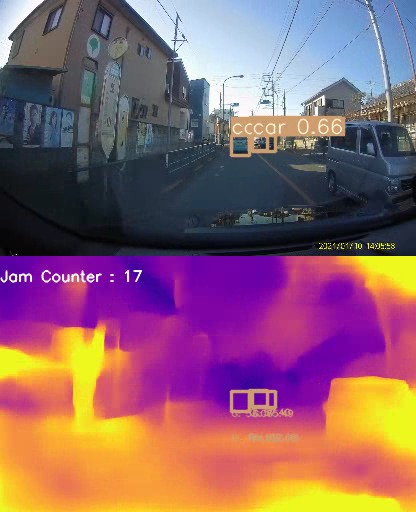
\includegraphics[width=4.5cm]{figs/ex01_01after.png}
    \end{center}
  \caption{結果1}
  \label{fig:ex01_01after}
\end{minipage}

  \begin{minipage}{0.33\hsize}
  \begin{center}
    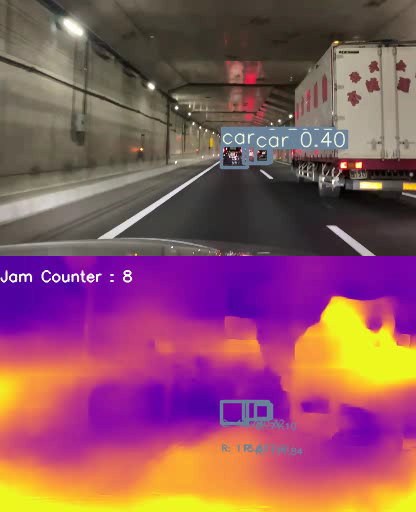
\includegraphics[width=4.5cm]{figs/ex01_02after.png}
  \end{center}
  \caption{結果2}
  \label{fig:ex01_02after}
\end{minipage}

  \begin{minipage}{0.33\hsize}
  \begin{center}
    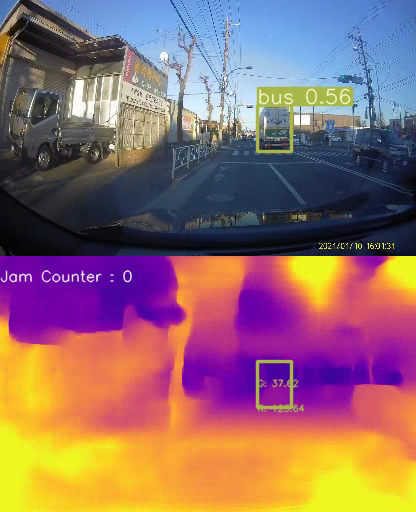
\includegraphics[width=4.5cm]{figs/ex01_03after.png}
  \end{center}
  \caption{結果3}
  \label{fig:ex01_03after}
\end{minipage}
\end{tabular}
\end{figure}
% ---------------------------------------------------

\figref{fig:ex01_01after},\figref{fig:ex01_02after}および\figref{fig:ex01_03after}からわかる通り,左右の1/3を検出しないことで先行車のみを検出し,より正しく渋滞推定を行うことができている.
また,実験1と実験2における動画の中で渋滞だと検出した回数の比較の表を以下に示す.

% ----------------------------------------------------
\begin{table}[htbp]
  \centering
  \begin{scriptsize}
  \begin{tabular}{ccc}
  \toprule
映像番号 & 実験1 & 実験2\\
  \midrule
映像1 & 425 & 131\\
映像2 & 1309 & 401\\
映像3 & 256 & 59\\
映像4 & 1364 & 65\\
  \bottomrule
  \end{tabular}
  \end{scriptsize}
  \caption{実験2 - 結果}
  \label{tab:dataset}
\end{table}
% ------------------------------------------------------
\newpage
\section{実験3 さまざまな状況における本システムの推定精度実験}
これまでの実験を通してシステムをさらに改良し、さまざまな状況下のドライブレコーダー映像を使って本システムの推定精度を測定する実験を行った。
これまでの実験に用いたデーターセットはどれも前方に先行車があるという状況だったが、この実験では先行車がない映像や信号で停止している映像を用いて本システムの推定精度に関して実験評価を行う。
実験3を行うにあたって人間の目で渋滞しているフレーム数を数える必要があるため、システムにおいて出力された映像の中央にフレーム数を明記されるように改良した。
また、本実験においては人間の目で渋滞を判断するにあたって、信号等の要素を排除し、車道において先行車が停止し、停止ランプがついており、ドライブレコーダーが取り付けられている自動車も停車している状況を渋滞と判断した。
%
%そのうえで、この実験が提案手法を評価する上で十分なのか、もう少し検討しましょう。
%少なくとも、各動画の渋滞状況をground truthとして示し、システムでの検出結果を示し、それらを比較する必要があります。
%これに加えて、全く渋滞していない、少し流れが悪い、断続的に渋滞、全く動いていない、みたいに、いろいろな状況の動画での実験が必要と思います。
%
%

\subsection{使用したデータセット}
本実験において使用したデータセットを以下の表に示す。

% ----------------------------------------------------
\begin{table}[htbp]
  \centering
  \begin{scriptsize}
  \begin{tabular}{cccccc}
  \toprule
映像番号 & 映像の内容 & 映像時間 & フレーム数 & 時間帯 & 道路 \\
  \midrule
映像1 & 全く渋滞していない & 60秒 & 1830フレーム & 昼 & 一般道 \\
映像2 & 先行車あり スムーズに進んでいる & 60秒 & 1830フレーム & 昼 & 一般道 \\
映像3 & 途中信号による停車あり & 60秒 & 1830フレーム & 昼 & 一般道 \\
映像4 & 渋滞中の継続的な渋滞 & 60秒 & 1830フレーム & 昼 & 一般道 \\
映像5 & 信号による停車 & 31秒& 928フレーム & 昼 & 一般道 \\
  \bottomrule
  \end{tabular}
  \end{scriptsize}
  \caption{実験3 データーセット}
  \label{tab:exp_dataset3}
\end{table}
% ------------------------------------------------------

\subsection{結果}
上記のデータセットを使い、本システムの推定精度を実験した。
また出力された数値をもとにmAP(mean Average Precision)値を求め、以下に示す。

% ----------------------------------------------------
\begin{table}[htbp]
  \centering
  \begin{scriptsize}
  \begin{tabular}{cccc}
  \toprule
映像番号 & 映像の内容 & システムの渋滞推定フレーム数 & 渋滞判断フレーム数(Ground Truth)\\
  \midrule
映像1 & 先行車なし 無渋滞 & 0 & 0 \\
映像2 & 先行車あり スムーズに進んでいる & 4 & 0 \\
映像3 & 途中信号による停車あり & 167 & 870\\
映像4 & 渋滞中の継続的な渋滞 & 130 & 452\\
映像5 & 信号による停車 & 251 & 927 \\
\bottomrule
\end{tabular}
\end{scriptsize}
  \caption{実験3 - 結果}
  \label{tab:exp3_fig}
\end{table}
% ------------------------------------------------------

\section{再現性 適合率 mAP}
本システムにおける再現性、適合率及びmAP値を測定するための実験を行った。
実験3にて出力された映像データー5つから、それぞれ20フレームずつ抽出し、合計100フレーム画像における再現性、適合率、mAPの値を調べた。
その結果を以下に示す。